\section{密度的计算与表示}
\label{sec:density-computation}

前两节回答了密度何时存在、怎样使用。本节回到具体测度，依次计算三类常见对象的密度：可数集合上的离散质量、由实轴函数增量产生的质量，以及经过映射后得到的推前测度。每个例子都先指明参考测度，再求密度，最后核对它能否恢复目标测度在集合上的质量。

\subsection{离散测度的密度}
\label{sec:density-discrete}

\paragraph{逐点相除}
设$X=\{x_1,x_2,\dots\}$是可数集合，取全部子集为可测集，参考测度与目标测度分别为
\[
 \mu=\sum_im_i\delta_{x_i},\qquad \nu=\sum_ip_i\delta_{x_i},\qquad m_i,p_i\in[0,+\infty).
\]
单点质量有限，可数个单点覆盖$X$，所以两者都$\sigma$有限。先检查绝对连续：$\mu(A)=0$当且仅当$A$中每点的$m_i$都为零，所以$\nu\ll\mu$当且仅当“$m_i=0$蕴含$p_i=0$”。在此条件下，令
\[
 h(x_i)=\frac{p_i}{m_i}\quad(m_i>0),\qquad h(x_i)\text{ 取任意非负值}\quad(m_i=0).
\]
对离散测度的积分是加权求和（第~\ref{sec:integral-classical}节），于是对任意$A\subseteq X$，
\[
 \int_Ah\,\mathrm d\mu=\sum_{x_i\in A}h(x_i)m_i=\sum_{x_i\in A,\,m_i>0}p_i=\sum_{x_i\in A}p_i=\nu(A),
\]
第三个等号用到$m_i=0$时$p_i=0$。因此$h$是$\nu$相对于$\mu$的密度。$m_i=0$的点是$\mu$零测集，密度在那里的取值可以任意，这正是第~\ref{sec:density-ae-version}小节的几乎处处版本。与长度测度不同，离散参考测度在每个正质量点上都允许逐点相除，第~\ref{sec:density-definition}小节有限点集上的质量之比在这里推广到了可数情形。

\paragraph{同一分布换两种参考}
在$\{0,1,2,\dots\}$上取参数为$1$的Poisson分布$p_k=\mathrm e^{-1}/k!$为目标。相对于计数测度，密度就是概率质量函数$p_k$本身。若改用几何权重$m_k=2^{-(k+1)}$作参考，所有$m_k>0$，密度为
\[
 h(k)=\frac{p_k}{m_k}=\frac{2^{k+1}\mathrm e^{-1}}{k!},
\]
前几项约为$0.736,1.472,1.472,0.981,0.491,0.196$。核对一个集合：$\nu(\{0,1\})=2\mathrm e^{-1}\approx0.7358$，而$h(0)m_0+h(1)m_1\approx0.7358\cdot0.5+1.4715\cdot0.25\approx0.7358$。两种密度之间由链式规则联系：几何权重相对于计数测度的密度是$m_k$，所以$h(k)\cdot m_k=p_k$。图~\ref{fig:density-discrete}画出了两组点质量及它们的比值。

\begin{figure}[!htbp]
  \centering
  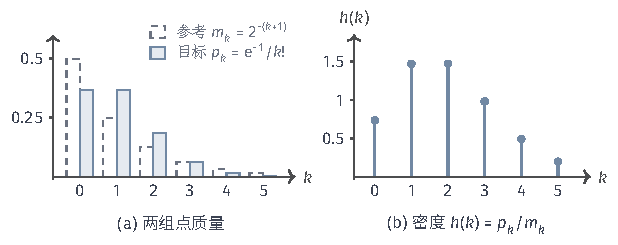
\includegraphics[width=104.712mm]{figures/02-abstract-mathematics/01-metric-and-measure/tikz/c4-discrete-density/figure.pdf}
  \caption{可数集合上的离散密度。(a)虚线框为几何参考质量$m_k=2^{-(k+1)}$，蓝色柱为Poisson目标质量$p_k=\mathrm e^{-1}/k!$，$k=0,\dots,5$。(b)密度$h(k)=p_k/m_k$：$k=1,2$处目标质量相对参考最多，$h$约为$1.47$；$k$增大后几何权重比阶乘倒数衰减得慢，$h$趋于零。}
  \label{fig:density-discrete}
\end{figure}

\paragraph{总质量}
密度的计算与总质量是否有限无关。仍以几何权重为参考，计数测度$\nu=\sum_k\delta_k$的密度是$h(k)=2^{k+1}$，$\nu$的总质量为$+\infty$，但每个有限集合上的质量都由$h$正确恢复。只有目标测度是概率测度时，才要求$\sum_kh(k)m_k=1$。

\subsection{增量测度的密度}
\label{sec:density-increment}

第~\ref{sec:integral-differentiation}节从函数一侧研究了增量：有界变差函数可以写成两个单调函数之差，绝对连续函数的增量可以由导数的积分恢复。本小节把函数增量变成集合上的质量，再问这个质量何时有Lebesgue密度。

\paragraph{由增量产生的有符号测度}
设$F:[a,b]\to\mathbb R$可以写成$F=F_1-F_2$，其中$F_1,F_2$单调不减且右连续。每个右连续的有界变差函数都有这样的分解：取$F_1(x)$为$F$在$[a,x]$上的总变差、$F_2=F_1-F$，二者单调不减（第~
ef{sec:integral-differentiation}节）；$F$右连续时$F_1$也右连续，这一点需要单独证明（可参照Folland《Real Analysis》第3.5节关于有界变差函数的讨论），本小节直接使用这一结论。把$F_j$延拓到$\mathbb R$，在$x<a$处取$F_j(a)$，在$x>b$处取$F_j(b)$，延拓后仍单调不减、右连续。由第~\ref{sec:measure-construction}节的Lebesgue–Stieltjes构造得到有限测度$\mu_{F_1},\mu_{F_2}$，它们都集中在$(a,b]$上。令
\[
 \eta_F(E)=\mu_{F_1}(E)-\mu_{F_2}(E),\qquad E\in\mathcal B((a,b]),
\]
则$\eta_F$是$(a,b]$上的有限有符号测度，并且对$a\le s<t\le b$有
\[
 \eta_F((s,t])=\bigl(F_1(t)-F_1(s)\bigr)-\bigl(F_2(t)-F_2(s)\bigr)=F(t)-F(s).
\]
称$\eta_F$为$F$的\term{增量测度}（increment measure）。区间取左开右闭，与右连续性配合：$\eta_F$给$(s,t]$的质量是右端点值减左端点值。$F(a)$本身不进入$\eta_F$，它是恢复$F$时需要单独记下的常数：$F(x)=F(a)+\eta_F((a,x])$。

$\eta_F$不依赖于分解的选择，理由是下面的唯一性：$(a,b]$上的两个有限有符号测度$\eta,\eta'$若在所有区间$(s,t]\subseteq(a,b]$上相等，则$\eta=\eta'$。事实上，由Jordan分解，$\eta^++\eta'^-$与$\eta'^++\eta^-$是两个有限测度，它们在这些区间上相等；区间族对交运算封闭（两个这样的区间之交是同类区间或空集），且生成$\mathcal B((a,b])$，$(a,b]$本身也在其中，由$\pi$-$\lambda$定理（定理~\ref{thm:measure-pi-lambda}），两个测度在全部Borel集上相等，移项即得$\eta=\eta'$。若$F=G_1-G_2$是另一种分解，两种做法得到的有符号测度在区间上都等于$F$的增量，所以相同。

\paragraph{绝对连续函数的增量测度}
函数的绝对连续（定义~\ref{def:integral-absolutely-continuous-function}）与测度的绝对连续（定义~\ref{def:measure-absolutely-continuous}）是分别定义的。下面的定理说明，对增量测度而言二者是同一件事，并且密度就是导数。

\begin{theorem}[增量测度的密度]
\label{thm:density-increment}
设$F:[a,b]\to\mathbb R$。
\begin{enumerate}
 \item 若$F$绝对连续，则$\eta_F$有定义，$|\eta_F|\ll\lambda$，并且$\eta_F(E)=\int_EF'\,\mathrm d\lambda$对一切$E\in\mathcal B((a,b])$成立，即$\mathrm d\eta_F/\mathrm d\lambda=F'$。
 \item 反之，若$F=F_1-F_2$如上，且$|\eta_F|\ll\lambda$，则$F$绝对连续。
\end{enumerate}
\end{theorem}

\begin{proof}
(1) 由第~\ref{sec:integral-differentiation}节，绝对连续函数的导数$F'$几乎处处存在且可积，并且由微积分基本定理（定理~\ref{thm:integral-ftc}），$F(x)=F(a)+\int_a^xF'(t)\,\mathrm dt$。令$F_1(x)=F(a)+\int_a^x(F')^+\,\mathrm dt$，$F_2(x)=\int_a^x(F')^-\,\mathrm dt$，它们单调不减且连续，$F=F_1-F_2$，所以$\eta_F$有定义。另一方面，$\eta(E)=\int_EF'\,\mathrm d\lambda$是$(a,b]$上的有限有符号测度，对$a\le s<t\le b$，
\[
 \eta((s,t])=\int_s^tF'(x)\,\mathrm dx=F(t)-F(s)=\eta_F((s,t]).
\]
由上一段的唯一性，$\eta=\eta_F$。由定理~\ref{thm:density-signed}，$|\eta_F|(E)=\int_E|F'|\,\mathrm d\lambda$，所以$|\eta_F|\ll\lambda$。

(2) 设$|\eta_F|\ll\lambda$。$\lambda$在$(a,b]$上有限，由定理~\ref{thm:density-signed}，存在可积函数$h$使$\eta_F(E)=\int_Eh\,\mathrm d\lambda$。于是对$x\in[a,b]$，
\[
 F(x)=F(a)+\eta_F((a,x])=F(a)+\int_a^xh(t)\,\mathrm dt .
\]
可积函数的不定积分绝对连续（第~\ref{sec:integral-differentiation}节），所以$F$绝对连续；再由(1)，$h=F'$ $\lambda$-几乎处处。
\end{proof}

定理把第~\ref{chap:integration}章的恢复公式$F(t)-F(s)=\int_s^tF'$改写成测度语言：增量测度相对于长度的密度是导数。函数一侧的“小区间组总长度小则增量总和小”，在测度一侧就成为“长度零测集上没有增量质量”。

\paragraph{一般情形：保留奇异增量}
若$F$只是右连续的有界变差函数，$\eta_F$未必相对于$\lambda$绝对连续。这时对Jordan分解的两部分$\eta_F^+,\eta_F^-$分别作相对于$\lambda$的Lebesgue分解，再对两个绝对连续部分用Radon–Nikodym定理，得到可积函数$h$与有限有符号测度$\eta_{\mathrm s}$，使
\[
 \eta_F(E)=\int_Eh\,\mathrm d\lambda+\eta_{\mathrm s}(E),
\]
其中$\eta_{\mathrm s}$是两个与$\lambda$相互奇异的有限测度之差。密度只表示其中的绝对连续增量，奇异增量由$\eta_{\mathrm s}$单独承担。

用第~\ref{sec:density-decomposition}小节的例子具体计算。在$[0,1]$上令
\[
 F(x)=\frac x2+\frac14\mathbf 1_{[1/2,1]}(x)+\frac14C(x),
\]
其中$C$是第~\ref{sec:measure-decomposition}节的Cantor函数。三项都单调不减且右连续，分别产生$\tfrac12\lambda$、$\tfrac14\delta_{1/2}$与$\tfrac14\mu_C$；它们的和在每个区间$(s,t]$上给出$F(t)-F(s)$，由唯一性，
\[
 \eta_F=\tfrac12\lambda|_{(0,1]}+\tfrac14\delta_{1/2}+\tfrac14\mu_C .
\]
这正是图~\ref{fig:density-lebesgue-form}中的测度，绝对连续部分的密度是$1/2$。从函数一侧看，$F'=1/2$在$[0,1]$上几乎处处成立：一次项的导数为$1/2$，阶跃项在$x\ne1/2$处导数为零，Cantor函数在Cantor集之外导数为零（第~\ref{sec:integral-differentiation}节）。于是$\int_0^1F'(x)\,\mathrm dx=\tfrac12$，而$F(1)-F(0)=1$。恢复公式遗漏的$\tfrac12$恰好由两部分组成：$x=1/2$处的跳跃$\tfrac14$，以及Cantor函数的连续增长$\tfrac14$。图~\ref{fig:density-increment}画出了这个$F$。

\begin{figure}[!htbp]
  \centering
  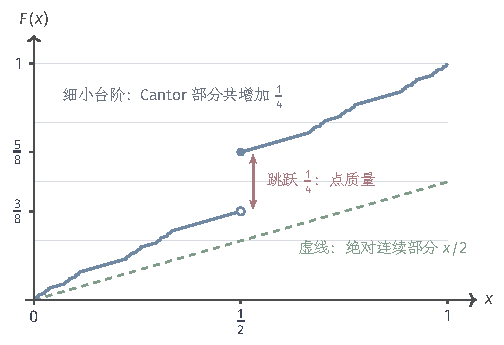
\includegraphics[width=85.425mm]{figures/02-abstract-mathematics/01-metric-and-measure/tikz/c4-increment-measure/figure.pdf}
  \caption{增量测度的三部分。蓝色曲线为$F(x)=x/2+\tfrac14\mathbf 1_{[1/2,1]}(x)+\tfrac14C(x)$，$C$为Cantor函数；绿色虚线$x/2$是绝对连续部分的累计，斜率$1/2$就是增量测度相对于长度的密度。$F$在$1/2$处从$3/8$跳到$5/8$（空心点为左极限，实心点为函数值），这$1/4$的增量是点质量；曲线上细小的台阶来自Cantor函数，它连续却在零长度的Cantor集上共增加$1/4$。曲线坐标在步长$1/243$的网格上计算。}
  \label{fig:density-increment}
\end{figure}

这个例子说明，“$F$连续”“$F$有界变差”“$F$几乎处处可导”都不足以保证增量测度有密度，必须要求绝对连续。把跳跃去掉后的$x/2+\tfrac14C(x)$已经连续，却仍有$\tfrac14$的奇异连续增量无法用密度表示。

\subsection{推前测度的密度}
\label{sec:density-pushforward}

随机变量经过一个函数变换后，分布变成推前测度（第~\ref{sec:measure-pushforward}节）。若输入测度有密度，输出测度是否有密度、怎样计算？第~\ref{sec:integral-change-of-variables}节已经建立了光滑换元公式，这里用它直接算出输出密度，不重复Jacobian公式的证明。

\paragraph{可逆光滑变换}
设$U,V\subseteq\mathbb R^d$是开集，$T:U\to V$是$C^1$微分同胚，即$T$可逆，且$T$与$T^{-1}$都连续可微。设$U$上的Borel测度$\mu$相对于$\lambda_d$有密度$p$。

\begin{theorem}[推前测度的密度]
\label{thm:density-pushforward}
在上述条件下，$T_\#\mu$相对于$V$上的$\lambda_d$有密度
\[
 q(\bm y)=p\bigl(T^{-1}(\bm y)\bigr)\,\bigl|\det DT^{-1}(\bm y)\bigr|,\qquad \bm y\in V .
\]
\end{theorem}

\begin{proof}
记$S=T^{-1}:V\to U$，它也是$C^1$微分同胚。把光滑换元公式（定理~\ref{thm:integral-jacobian-change}）用于$S$，对$U$上的非负可测函数$g$有
\[
 \int_Ug(\bm x)\,\mathrm d\bm x=\int_Vg\bigl(S(\bm y)\bigr)\,\bigl|\det DS(\bm y)\bigr|\,\mathrm d\bm y .
\]
对Borel集$B\subseteq V$，由推前测度的定义和密度的定义，
\[
 T_\#\mu(B)=\mu\bigl(T^{-1}(B)\bigr)=\int_U\mathbf 1_B\bigl(T(\bm x)\bigr)p(\bm x)\,\mathrm d\bm x .
\]
取$g(\bm x)=\mathbf 1_B(T(\bm x))p(\bm x)$，则$g(S(\bm y))=\mathbf 1_B(\bm y)p(S(\bm y))$，代入上式得
\[
 T_\#\mu(B)=\int_Bp\bigl(S(\bm y)\bigr)\,\bigl|\det DS(\bm y)\bigr|\,\mathrm d\bm y .
\]
\end{proof}

公式中的$|\det DT^{-1}(\bm y)|=1/|\det DT(T^{-1}(\bm y))|$度量了$T$在原像附近把体积压缩或拉伸的倍数：体积被拉伸的地方，同样多的质量摊到更大的范围，密度就变小。一维例子：$(0,1)$上的均匀概率$p=1$经$T(x)=-\ln x$映到$(0,+\infty)$，$T^{-1}(y)=\mathrm e^{-y}$，$|(T^{-1})'(y)|=\mathrm e^{-y}$，所以输出密度$q(y)=\mathrm e^{-y}$，即指数分布，$\int_0^\infty\mathrm e^{-y}\,\mathrm dy=1$。仿射变换$T(\bm x)=\bm A\bm x+\bm b$（$\bm A$可逆）给出$q(\bm y)=p(\bm A^{-1}(\bm y-\bm b))/|\det\bm A|$。

\paragraph{分支相加}
许多变换不是整体可逆的，例如$T(x)=x^2$把$x$与$-x$送到同一点。按第~\ref{sec:integral-change-of-variables}节分支换元的方式处理：设$U_1,U_2,\dots$是$U$中有限或可数个两两不交的开集，$U\setminus\bigcup_kU_k$是Lebesgue零测集，$T$在每个$U_k$上的限制$T_k:U_k\to V_k$是到开集$V_k$的$C^1$微分同胚，$S_k=T_k^{-1}$。因为$\mu\ll\lambda_d$，未纳入分支的部分也是$\mu$零测集。对Borel集$B$，
\[
 T_\#\mu(B)=\sum_k\mu\bigl(T^{-1}(B)\cap U_k\bigr)=\sum_k\int_{V_k}\mathbf 1_B(\bm y)\,p\bigl(S_k(\bm y)\bigr)\,\bigl|\det DS_k(\bm y)\bigr|\,\mathrm d\bm y,
\]
每一项用的是定理~\ref{thm:density-pushforward}的计算。被加项非负，由单调收敛定理可交换求和与积分，所以$T_\#\mu$的密度为
\[
 q(\bm y)=\sum_k\mathbf 1_{V_k}(\bm y)\,p\bigl(S_k(\bm y)\bigr)\,\bigl|\det DS_k(\bm y)\bigr| .
\]
各分支的像$V_k$可以重叠；在重叠处，所有原像分支的贡献都要累加。只取一个逆分支会遗漏质量。

\paragraph{平方变换}
取$[-1,1]$上的均匀概率测度，密度$p=1/2$，$T(x)=x^2$。两个分支是$U_1=(0,1)$与$U_2=(-1,0)$，未纳入的$\{-1,0,1\}$是零测集；两支的像都是$V_1=V_2=(0,1)$，逆映射$S_1(y)=\sqrt y$，$S_2(y)=-\sqrt y$，导数绝对值都是$1/(2\sqrt y)$。两支相加，
\[
 q(y)=\frac12\cdot\frac1{2\sqrt y}+\frac12\cdot\frac1{2\sqrt y}=\frac1{2\sqrt y},\qquad 0<y<1,
\]
在$(0,1)$外$q=0$。检查总质量：$\int_0^1\frac1{2\sqrt y}\,\mathrm dy=\bigl[\sqrt y\bigr]_0^1=1$。再核对一个集合：$B=[0.36,0.49]$的原像是$[-0.7,-0.6]\cup[0.6,0.7]$，输入质量为$0.2\times\tfrac12=0.1$；用输出密度计算，$\int_{0.36}^{0.49}\frac1{2\sqrt y}\,\mathrm dy=0.7-0.6=0.1$。若只取正分支，得到的$1/(4\sqrt y)$总积分只有$1/2$。

输出密度在$y\to0$时无界，但仍可积，所以原点附近的质量趋于零。原点的原像只有单点$\{0\}$，输入质量为$0$，故$T_\#\mu(\{0\})=0$，输出没有额外的点质量。若输入在$0$处有点质量，例如$\tfrac12\lambda|_{[-1,1]}$换成$\tfrac12\delta_0+\tfrac14\lambda|_{[-1,1]}$，推前后就会在$0$处出现点质量$\tfrac12$，这部分不能用相对于长度的密度表示。图~\ref{fig:density-square-branches}对照了输入端的两个原像区间与输出端的面积。

\begin{figure}[!htbp]
  \centering
  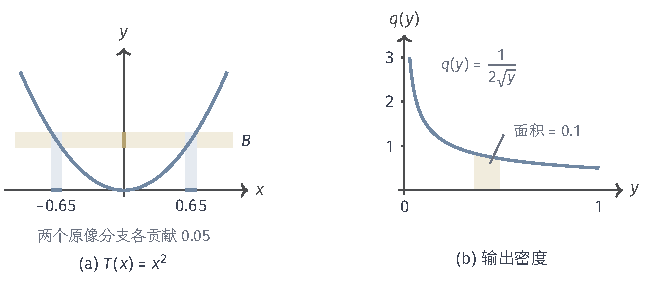
\includegraphics[width=110.144mm]{figures/02-abstract-mathematics/01-metric-and-measure/tikz/c4-square-branches/figure.pdf}
  \caption{平方变换下推前测度的密度。(a)$[-1,1]$上的均匀概率经$T(x)=x^2$映到$[0,1]$；输出区间$B=[0.36,0.49]$（黄色带）有两个原像分支$[-0.7,-0.6]$与$[0.6,0.7]$（蓝色条），各贡献质量$0.05$。(b)两支相加得到的输出密度$q(y)=1/(2\sqrt y)$，$B$上的面积为$0.1$，与输入端的质量一致；曲线在$y=1/36$处截断，$y\to0$时无界但可积。}
  \label{fig:density-square-branches}
\end{figure}
